\documentclass{standalone}

\usepackage{tikz}
\usetikzlibrary{positioning}

\tikzstyle{block} = [draw, fill=white, rectangle,
    minimum width=1.5cm, minimum height=7mm, 
    inner sep=0pt, outer sep=0pt
    ]

\tikzstyle{func} = [draw, fill=white, circle,
    minimum size=0.75cm, 
    inner sep=0pt, outer sep=0pt
    ]

\begin{document}
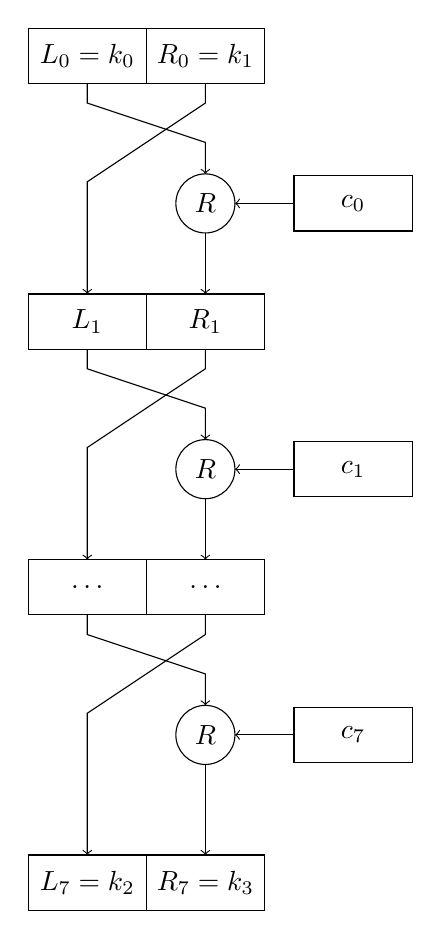
\begin{tikzpicture}[node distance=0cm]
    \newcommand{\len}{1.5cm}
    % Round 0
    \node [block] (R0) {$R_0 = k_1$};
    \node [block, left=of R0.west] (L0) {$L_0 = k_0$};
    \node [func, below of=R0, node distance=1.25*\len] (r0) {$R$};
    \node [block, right of=r0, node distance=1.25*\len] (c0) {$c_0$};
    % Round 1
    \node [block, below of=r0, node distance=\len] (R1) {$R_1$};
    \node [block, left=of R1.west] (L1) {$L_1$};
    \node [func, below of=R1, node distance=1.25*\len] (r1) {$R$};
    \node [block, right of=r1, node distance=1.25*\len] (c1) {$c_1$};
    % Round i
    \node [block, below of=r1, node distance=\len] (Ri) {$\ldots$};
    \node [block, left=of Ri.west] (Li) {$\ldots$};
    \node [func, below of=Ri, node distance=1.25*\len] (ri) {$R$};
    \node [block, right of=ri, node distance=1.25*\len] (ci) {$c_7$};
    % Round 8
    \node [block, below of=ri, node distance=1.25*\len] (R7) {$R_7=k_3$};
    \node [block, left=of R7.west] (L7) {$L_7=k_2$};
    %\node [func, below of=R7, node distance=\len] (r7) {$R$};
    %\node [block, right of=r7, node distance=1.25*\len] (c7) {$c_7$};

    % Round 0
    \draw [->] (R0.south) -- ++(0,-0.25) -- ++(-1.5, -1) -| (L1.north);
    \draw [->] (L0.south) -- ++(0,-0.25) -- ++(1.5,-0.5) -| (r0.north);
    \draw [->] (r0.south) -- (R1.north);
    \draw [->] (c0.west) -- (r0.east);
    % Round 1
    \draw [->] (R1.south) -- ++(0,-0.25) -- ++(-1.5, -1) -| (Li.north);
    \draw [->] (L1.south) -- ++(0,-0.25) -- ++(1.5,-0.5) -| (r1.north);
    \draw [->] (r1.south) -- (Ri.north);
    \draw [->] (c1.west) -- (r1.east);
    % Round 7
    \draw [->] (Ri.south) -- ++(0,-0.25) -- ++(-1.5, -1) -| (L7.north);
    \draw [->] (Li.south) -- ++(0,-0.25) -- ++(1.5,-0.5) -| (ri.north);
    \draw [->] (ri.south) -- (R7.north);
    \draw [->] (ci.west) -- (ri.east);
\end{tikzpicture}
\end{document}